\documentclass{beamer}
\usetheme{metropolis}

\usepackage{graphicx}
\usepackage{tikz}
\usepackage{caption}
\usepackage{adjustbox}
\usepackage{listings}
\usepackage{wrapfig}
\usepackage{color}
\usepackage{listings}
\usepackage{pgfpages}
\setbeameroption{show notes on second screen=right}

\usetikzlibrary{automata,positioning,shapes,snakes}
\usetikzlibrary{calc,matrix,arrows,automata,decorations.pathmorphing}
\usetikzlibrary{shapes.geometric, arrows.meta, positioning}
\pgfmathtruncatemacro\distance{1}


\lstset{language=erlang, basicstyle=\sffamily\footnotesize,
  keywordstyle=\color{blue}, numberstyle=\tiny, numbers=none,
  showspaces=false, showstringspaces=false, frame=tL, mathescape=true,
  backgroundcolor=\color{black!5}, morekeywords={send, to, from} }


\title{Choreographies for Program Understanding}
\author{\textbf{Gabriele Genovese}, Ivan Lanese, Cinzia Di Giusto, Emilio Tuosto,
and Germ\'an Vidal}
\date{17 June 2025}

\begin{document}


% title
\maketitle
\note{
  Good afternoon, everyone. Today I’m presenting our work titled
  “Choreographies for Program Understanding,” developed in collaboration
  with Ivan Lanese, Cinzia Di Giusto, Emilio Tuosto, and Germán Vidal.
  This work is about analyzing distributed systems from a global
  perspective, even when we only have access to the local code with
  an ad-hoc extraction techniques.
  Let’s start by looking at the big picture of distributed systems.
}

% slide 1

\begin{frame}{Distributed Systems are Hard}
Abstractions in order to simplify:

\bigskip

\tikzstyle{box} = [rectangle, rounded corners, draw=blue!60, fill=blue!10, thick,
                   text width=7.5em, text centered, minimum height=2em]

\centering
\begin{tikzpicture}[node distance=1cm]
\node (ind) [box] {Actor model\\(industry)};
\node (sci) [box, right=of ind] {Choreographies\\(research)};
\draw[->] (sci) -- (ind);
\draw[->] (ind) -- (sci);
\end{tikzpicture}
\end{frame}
\note{
Distributed systems are complex by nature.
To manage this complexity, we rely on abstractions
that help structure and reason about interactions.
In industry, the actor model is commonly used—think Erlang or Akka.
Meanwhile, in academia, we focus on choreographies,
which give a global view of the system behavior.
In this talk, I’ll show how we bridge these two views.
}

% slide 2

\begin{frame}{The Actor Model}
\begin{columns}
\column{0.48\textwidth}
\begin{block}{Main concepts}
\begin{itemize}
    \item Process with mailbox
    \item Asynchronous messaging
\end{itemize}
\end{block}
\column{0.48\textwidth}
\begin{figure}
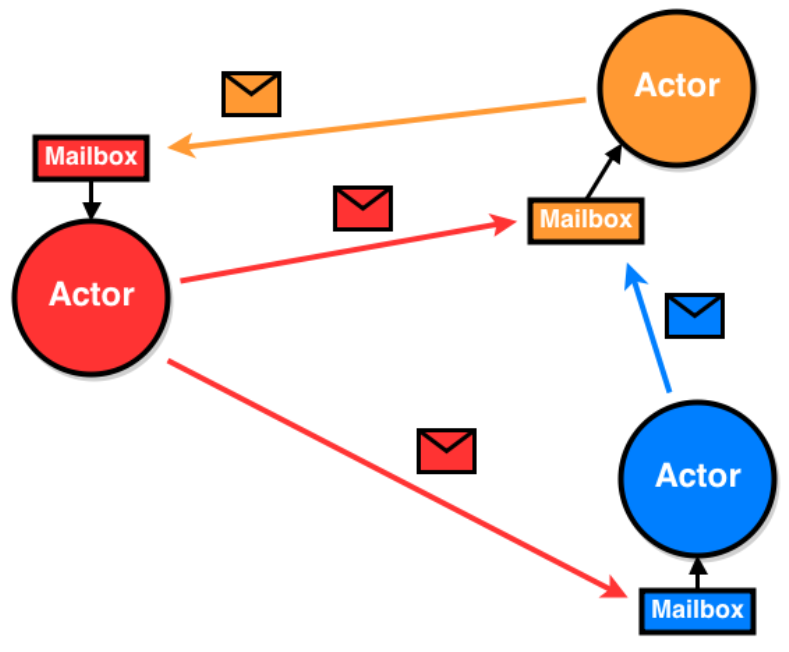
\includegraphics[width=1.1\textwidth]{images/actors.png}
\end{figure}
\end{columns}
\end{frame}
\note{
  Let’s start with the actor model.
  Each actor is an independent process with its own mailbox.
  They interact purely by sending and receiving messages asynchronously.
  This model scales well and fits naturally into distributed environments.
}

% slide 3
\begin{frame}{The Actor Model}
\begin{columns}
\column{0.48\textwidth}
\begin{block}{Ecosystem}
\begin{itemize}
    \item Erlang, Elixir, Scala
    \item Akka (Java), Actix (Rust)
    \item Go routines and channels
\end{itemize}
\end{block}
\column{0.48\textwidth}
\begin{figure}

\includegraphics[width=\textwidth]{images/pl.png}
\end{figure}
\end{columns}
\end{frame}
\note{
  The actor model has strong practical support.
  Languages like Erlang, Elixir, and Scala adopt it directly.
  Frameworks like Akka for Java and Actix for Rust are built around it.
  Even Go, although not actor-based, has a similar concurrency model
  using goroutines and channels.
}

% slide 4
\begin{frame}{Choreography Automata \small{[1]}}
\begin{columns}
\column{0.48\textwidth}
\begin{block}{Informally}
\begin{itemize}
    \item Choreography: describes distributed protocols
    \item Paired with automata theory
\end{itemize}
\end{block}
\column{0.45\textwidth}
\begin{figure}
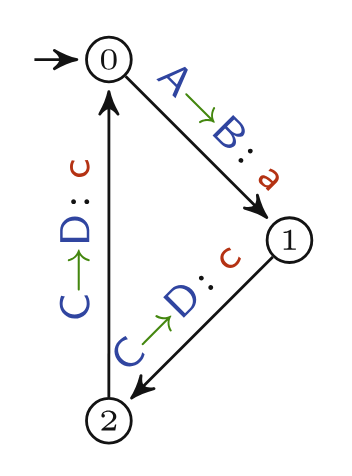
\includegraphics[width=0.9\textwidth]{images/chorauto.png}
\end{figure}
\end{columns}
\vspace{0.5em}
{\tiny [1] Barbanera et al. "Choreography automata." COORDINATION, 2020.}
\end{frame}
\note{
  In research, we often take a more global view of communication.
  A choreography describes all the participants and their interactions
  from a central perspective.
  By pairing this with automata theory, we can rigorously define
  and analyze these protocols.
  This idea was formalized in “Choreography Automata”
  by Barbanera et al.
}


\tikzset{
  state/.style={
	 inner sep=3pt,
	 minimum size = 6pt,
	 draw,
	 circle,
	 font=\scriptsize,
	 transform shape
  },
  mylabel/.style={
	 font=\tiny,
	 sloped,
	 above
  }
}

% slide 5
\begin{frame}{Global vs Local View}
\begin{columns}
\column{0.48\textwidth}
\begin{block}{Global}
\vspace{2em}
\begin{center}
\begin{tikzpicture}[node distance=2cm, transform shape]
	\node[state] (n_1) {1};
	\node[state] (n_2) [right of=n_1] {2};
	\node[state,accepting] (n_3) [right of=n_2] {3};
	
	\draw[->] (n_1) edge[bend left=0] node[mylabel] {A→B:hello} (n_2);
	\draw[->] (n_2) edge[bend left=0] node[mylabel] {B→A:hi} (n_3);
\end{tikzpicture}
\end{center}
\note{
  Choreographies offer both a global view—where we see all interactions—
  and local views, where each participant sees only their own role.
  For example, if A sends “hello” to B and B replies “hi”,
  the global view captures the full exchange.
  Locally, A just sees “send hello”, and B just sees “receive hello,
  then send hi”.
  Translating between these two views is key to our work.
}
	
\bigskip
The communication system is seen as a whole.

\end{block}
\column{0.48\textwidth}
\begin{block}{Local}
\begin{center}
\begin{tikzpicture}[node distance=1.5cm, transform shape]
	\node[state, draw=none] (n_0) [left of=n_1,node distance=0.8cm] {A:};
	\node[state] (n_1) {1};
	\node[state] (n_2) [right of=n_1] {2};
	\node[state,accepting] (n_3) [right of=n_2] {3};
	\node[state, draw=none] (n_10) [below of=n_0] {B:};
	\node[state] (n_4) [below of=n_1] {1};
	\node[state] (n_5) [right of=n_4] {2};
	\node[state,accepting] (n_6) [right of=n_5] {3};
	
	\draw[->] (n_1) edge[bend left=0] node[mylabel] {!B:hello} (n_2);
	\draw[->] (n_2) edge[bend left=0] node[mylabel] {?B:hi} (n_3);

	\draw[->] (n_4) edge[bend left=0] node[mylabel] {?A:hello} (n_5);
	\draw[->] (n_5) edge[bend left=0] node[mylabel] {!A:hi} (n_6);
\end{tikzpicture}
\end{center}
	
An actor’s individual perspective.

\end{block}
\end{columns}
\end{frame}

% slide 6
\begin{frame}{Top-Down Approach}
\textbf{Steps:}
\begin{enumerate}
  \item Write the global specification
  \item Project to obtain the local specification
  \item Write the local functions that respect the specification
\end{enumerate}
\textbf{Problem:} no way to include existing code and architecture.
\end{frame}
\note{
  One classical approach is top-down:
  You write a global choreography, project it to get local specifications,
  and implement those locally.
  However, this doesn’t work well if you’re dealing with existing systems
  or legacy code—you can’t easily inject a top-down design after the fact.
}

% slide 7
\begin{frame}{Aim}
\centering
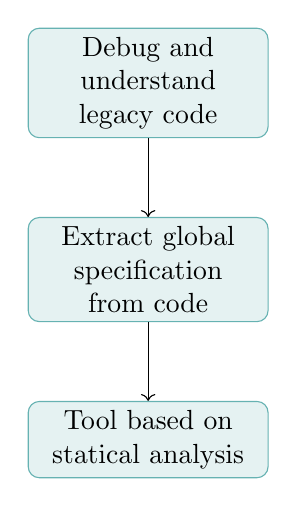
\begin{tikzpicture}[
    node distance=1cm,
    block/.style={rectangle, draw=teal!60, fill=teal!10, rounded corners,
                  text width=8em, align=center, minimum height=2em}]
\node[block] (bridge) {Debug and understand legacy code};
\node[block, below=of bridge] (extract) {Extract global specification from code};
\node[block, below=of extract] (tool) {Tool based on statical analysis};

\draw[->] (bridge) -- (extract);
\draw[->] (extract) -- (tool);
\end{tikzpicture}
\end{frame}
\note{
  Our aim is different:
  We want to understand and debug legacy systems.
  The idea is to extract a global view from already written code.
  We’re building a tool to do this using static analysis,
  starting from real programs.
}

% slide 8
\begin{frame}{Bottom-up approach}
\textbf{Extraction steps:}
\begin{enumerate}
  \item Analyze an input source code
  \item Create the local view
  \item Combine the local view to create an approximation global view
\end{enumerate}
\end{frame}
\note{
  So instead of top-down, we use a bottom-up approach:
  First, we analyze the code to extract local views.
  Then, we combine them to build an approximate global view.
  It’s not perfect, but it can already tell us a lot—
  especially when we care about communication behavior.
}

% slide 9
\begin{frame}{Why}
\begin{columns}
\column{0.5\textwidth}
\begin{block}{Benefits}
\begin{itemize}
  \item Highlights bugs (deadlock, race condition, etc...)
  \item Improves understanding of the code: give also good behavior
  % \item Educational potential
\end{itemize}
\end{block}
\column{0.5\textwidth}
\includegraphics[width=\linewidth]{example-image-a}
\end{columns}
\end{frame}
\note{
  Why go through all this effort?
  Well, the extracted models can reveal bugs like deadlocks
  or race conditions.
  But they also show correct behaviors—
  they help us understand what the code actually does.
  This is helpful both for developers and educators
  working on distributed algorithms.
}

% slide 10
\begin{frame}{Requirements}
\begin{itemize}
  \item Automatic extraction using bottom-up and over-approximation techniques
  \item Capture good behaviors and highlight misbehavior
  \item Support multiple actors
  \item Target mainstream language
  \item Simple notation
\end{itemize}
\end{frame}
\note{
  To make this useful in practice, we need several things:
  First, the process should be automatic,
  using static analysis and over-approximation.
  It should highlight both good and bad behaviors,
  support multiple actors,
  and be applicable to mainstream languages.
  Finally, the output should be easy to read—
  something people can reason with.
}

% slide 11
\begin{frame}{Problems}
\begin{itemize}
    \item Undecidability: we should decide termination
    \item Huge descriptions: given the over-approximation approach
\end{itemize}
\end{frame}
\note{
  Naturally, there are challenges.
  One is undecidability: we can’t always determine termination
  or correctness.
  Another is that over-approximations can lead to very large models,
  which can be hard to manage.
  So the trick is to balance precision and scalability.
}

\begin{frame}{Motivating Examples}
\textbf{Two example:}

\bigskip

\centering
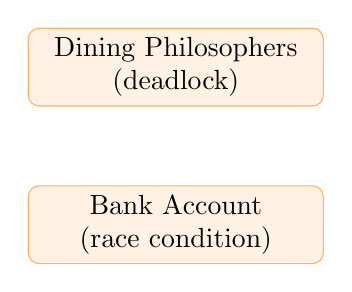
\begin{tikzpicture}[
    example/.style={rectangle, draw=orange!60, fill=orange!10, rounded corners,
                    text width=10em, align=center, minimum height=2em}]
\node[example] (philo) {Dining Philosophers\\(deadlock)};
\node[example, below=1cm of philo] (bank) {Bank Account\\(race condition)};

% \draw[->] (philo) -- (bank);
\end{tikzpicture}
\end{frame}

\begin{frame}[fragile]{Deadlock}
\begin{figure}[t]
  \centering
	 \begin{tikzpicture}[node distance=2cm, transform shape]
        \node[state] (n_1) {1};
        \node[state] (n_2) [above right of=n_1] {2};
        \node[state] (n_3) [below right of=n_1, fill=red] {3};
        
        \draw[->] (n_1) edge[bend left=0] node[mylabel] {A→B:error} (n_3);
        \draw[->] (n_1) edge[bend left=25] node[mylabel] {A→B:req} (n_2);
        \draw[->] (n_2) edge[bend left=25] node[mylabel] {B→A:res} (n_1);
      \end{tikzpicture}
  \caption{A deadlock can occur if a non-final state without outgoing transitions is present.}
  \label{fig:deadlock}
\end{figure}
\end{frame}

\begin{frame}[fragile]{Dining Philosophers example}
\begin{columns}
\column{0.53\textwidth}
\begin{lstlisting}
philosopher(Fork1, Fork2) $\to$
  send req to Fork1,
  receive ack from Fork1,
  send req to Fork2,
  receive ack from Fork2,
  eat(),
  send release to Fork1,
  send release to Fork2,
  philosopher(Fork1, Fork2).

fork() $\to$
  receive req from Phil,
  send ack to Phil,
  receive release from Phil,
  fork().
\end{lstlisting}
\column{0.46\textwidth}
\textbf{Participants:}
\begin{itemize}
  \item 2 philosophers
  \item 2 forks
\end{itemize}
\bigskip

\centering
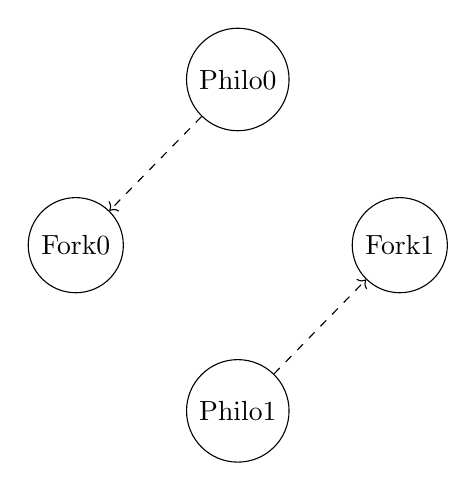
\begin{tikzpicture}
\node[state] (philo0) {Philo0};
\node[state,below=1cm of philo0, draw=none] (hidden) {};
\node[state,left=1 of hidden] (fork0) {Fork0};
\node[state,right=1 of hidden] (fork1) {Fork1};
\node[state,below=1cm of hidden] (philo1) {Philo1};

\draw[->,style=dashed] (philo0) -- (fork0);
\draw[->,style=dashed] (philo1) -- (fork1);
\end{tikzpicture}
\end{columns}
\end{frame}


\begin{frame}[fragile]{Dining Philosophers global-view}
\begin{figure}[t]
  \centering
	 \begin{tikzpicture}[node distance=2.5cm and .5cm, transform shape]
        \node[state] (n_1) {1};
        \node[state] (n_5) [below of=n_1, yshift=1cm, fill=red] {5};
        \node[state] (n_2) [right of=n_5] {2};
        \node[state] (n_3) [left of=n_5] {3};
        \node[state] (n_4) [right of=n_2] {4};
        \node[state] (n_6) [left of=n_3] {6};
        
        \draw[->] (n_1) edge[bend left=5] node[mylabel] {philo0→fork0:req} (n_2);
        \draw[->] (n_1) edge[bend right=5]  node[mylabel] {philo1→fork1:req} (n_3);
        \draw[->] (n_2) -- node[mylabel] {philo1→fork1:req} (n_5);
        \draw[->] (n_3) -- node[mylabel] {philo0→fork0:req} (n_5);
        \draw[->] (n_2) -- node[mylabel] {philo0→fork1:req} (n_4);
        \draw[->] (n_4) edge[bend right=20] node[mylabel] {philo0→fork\{0,1\}:release} (n_1);
        \draw[->] (n_3) -- node[mylabel] {philo1→fork0:req} (n_6);
        \draw[->] (n_6) edge[bend left=20] node[mylabel] {philo1→fork\{0,1\}:release} (n_1);
      \end{tikzpicture}
  \caption{Global view of the dining philosophers example.}
  \label{graph:philosophers}
\end{figure}
\end{frame}


\begin{frame}[fragile]{Bank account example}
\begin{columns}
\column{0.53\textwidth}
\begin{lstlisting}
account(Value) $\to$
  receive
    read from Client $\to$
	send Value to Client,
	account(Value);
    NewValue from Client $\to$
      account(NewValue).

client() $\to$
  send read to Acc,
  receive Value from Acc,
  % operations on Value
  send NewValue to Acc.
\end{lstlisting}
\column{0.46\textwidth}
\textbf{Participants:}
\begin{itemize}
  \item 1 account
  \item 2 clients
\end{itemize}

\bigskip

\centering
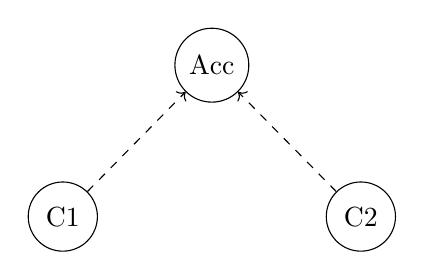
\begin{tikzpicture}
\node[state] (acc) {Acc};
\node[state,below=1cm of acc, draw=none] (hidden) {};
\node[state,left=1 of hidden] (c1) {C1};
\node[state,right=1 of hidden] (c2) {C2};

\draw[->,style=dashed] (c1) -- (acc);
\draw[->,style=dashed] (c2) -- (acc);
\end{tikzpicture}
\end{columns}
\end{frame}

\newcommand\dummy{C}
\tikzset{
	hpath/.style={
			very thick,
			line cap = round,
			line join = round,
			line width=0.1cm,
			opacity=.70,
			color = teal!30
		}
}
\begin{frame}[fragile]{Bank account global-view}
\begin{figure}[h!]
	\centering
	\begin{tikzpicture}[node distance={27mm}, scale = .6, transform shape, thick, main/.style = {draw, circle}]
		\node (n_1) [state] {\phantom{11}};
		\node (n_2) [state, below left of=n_1] {\phantom{11}};
		\node (n_3) [state, below right of=n_1] {\phantom{11}};
		\node (n_4) [state, left= 3.5cm of n_2] {4};
		\node (n_5) [state, below=3cm of n_1] {\phantom{11}};
		\node (n_6) [state, right= 3.5cm of n_3] {6};
		\node (n_7) [state, below of=n_4] {7};
		\node (n_8) [state, below left of=n_5] {\phantom{11}};
		\node (n_9) [state, below right of=n_5] {\phantom{11}};
		\node (n_10) [state, below of=n_6] {10};
		\node (n_11) [state, accepting, below= of n_7] {11};
		\node (n_12) [state, accepting, below=1.5cm of n_8] {\phantom{12}};
		\node (n_13) [state, accepting, below= 1.5cm of n_9] {\phantom{13}};
		\node (n_14) [state, accepting, below=2.5cm of n_10] {14};

		\draw[->] (n_1) -- node[midway, above left] {acc→\dummy1:Value} (n_2);
		\draw[->] (n_2) -- node[midway, below left] {acc→\dummy2:Value} (n_5);
		\draw[->] (n_5) -- node[midway, above left=-2mm] {\dummy1→acc:NewValue} (n_8);
		\draw[->] (n_8) -- node[midway, below left] {\dummy2→acc:NewValue} (n_12);

		\draw[->] (n_1) -- node[midway, above right] {acc→\dummy2:Value} (n_3);
		\draw[->] (n_3) -- node[midway, below right] {acc→\dummy1:Value} (n_5);
		\draw[->] (n_5) -- node[midway, above right=-2mm] {\dummy2→acc:NewValue} (n_9);
		\draw[->] (n_9) -- node[midway, below right] {\dummy1→acc:NewValue} (n_13);

		\draw[hpath] ($(n_1.center) + (-5pt,-5pt)$) -- (n_2.center) -- (n_5.north west) -- ($(n_5.center)+(-5pt,0)$) -- (n_5.south west) -- (n_8.center) -- ($(n_12.center) + (0pt,5pt)$);
		\draw[hpath] ($(n_1.center) + (5pt,-5pt)$) -- (n_3.center) -- (n_5.north east)  -- ($(n_5.center)+(5pt,0)$) -- (n_5.south east)  -- (n_9.center) -- ($(n_13.center) + (0pt,5pt)$);

		\foreach \n in {1,2,3,5,8,9,12,13}{
				\node at (n_\n) {\n};
			}

		\draw[->] (n_2) -- node[midway, above=3mm] {C1→acc:NewValue} (n_4);
		\draw[->] (n_4) -- node[midway, above left] {acc→C2:Value} (n_7);
		\draw[->] (n_7) -- node[midway, above left] {C2→acc:NewValue} (n_11);

		\draw[->] (n_3) -- node[midway, above=3mm] {C2→acc:NewValue} (n_6);
		\draw[->] (n_6) -- node[midway, above right] {acc→C1:Value} (n_10);
		\draw[->] (n_10) -- node[midway, above right] {C1→acc:NewValue} (n_14);
	\end{tikzpicture}
	\caption{Global view of the bank account example}
	\label{fig:account}
\end{figure}
\end{frame}

\begin{frame}{Conclusion}
\begin{block}{Summary}
\begin{itemize}
  \item Problem: no way to express legacy code
	\item Bridge the gap between programming and theoretical frameworks
	\item Use of bottom-up and over-approx techniques
\end{itemize}
\end{block}
\textbf{Future work:} create the tool as described ({\color{red}WIP}) 
and evaluate it on real-world examples.
\end{frame}

% \begin{frame}{Future Work}
% \begin{itemize}
% 	\item WIP on a tool called Chorer
% \end{itemize}
% \end{frame}

\begin{frame}{}
\centering
\Huge Thanks for listening!
\end{frame}


\end{document}
